%%%%%%%%%%%%%%%%%%%%%%%%%%%%%%%%%%%%%%%%%%%%%%%%%%%%%%%%%%%%%%%%%%%%%%%
%
%  A small sample UNSW Honours Thesis file.
%  Any questions to Ian Doust i.doust@unsw.edu.au
%
% Edited CSG 11.9.2015, use some of Gery's ideas for front matter; add a conclusion chapter.
%%%%%%%%%%%%%%%%%%%%%%%%%%%%%%%%%%%%%%%%%%%%%%%%%%%%%%%%%%%%%%%%%%%%%%%
%
%  The first part pulls in a UNSW Thesis class file.  This one is
%  slightly nonstandard and has been set up to do a couple of
%  things automatically
%
 
\documentclass[honours,12pt]{unswthesis}
\linespread{1}
\usepackage{cite}
\usepackage{amsfonts}
\usepackage{amssymb}
\usepackage{amsthm}
\usepackage{amsmath}
\usepackage{latexsym,amsmath}
\usepackage{graphicx}
\usepackage{afterpage}
\usepackage{tabularx}

%%%%%%%%%%%%%%%%%%%%%%%%%%%%%%%%%%%%%%%%%%%%%%%%%%%%%%%%%%%%%%%%%
%
%  The following are some simple LaTeX macros to give some
%  commonly used letters in funny fonts. You may need more or less of
%  these
%
\newcommand{\R}{\mathbb{R}}
\newcommand{\Q}{\mathbb{Q}}
\newcommand{\C}{\mathbb{C}}
\newcommand{\N}{\mathbb{N}}
\newcommand{\F}{\mathbb{F}}
\newcommand{\PP}{\mathbb{P}}
\newcommand{\T}{\mathbb{T}}
\newcommand{\Z}{\mathbb{Z}}
\newcommand{\B}{\mathfrak{B}}
\newcommand{\BB}{\mathcal{B}}
\newcommand{\M}{\mathfrak{M}}
\newcommand{\X}{\mathfrak{X}}
\newcommand{\Y}{\mathfrak{Y}}
\newcommand{\CC}{\mathcal{C}}
\newcommand{\E}{\mathbb{E}}
\newcommand{\cP}{\mathcal{P}}
\newcommand{\cS}{\mathcal{S}}
\newcommand{\A}{\mathcal{A}}
\newcommand{\ZZ}{\mathcal{Z}}
%%%%%%%%%%%%%%%%%%%%%%%%%%%%%%%%%%%%%%%%%%%%%%%%%%%%%%%%%%%%%%%%%%%%%
%
% The following are much more esoteric commands that I have left in
% so that this file still processes. Use or delete as you see fit
%
\newcommand{\bv}[1]{\mbox{BV($#1$)}}
\newcommand{\comb}[2]{\left(\!\!\!\begin{array}{c}#1\\#2\end{array}\!\!\!\right)
}
\newcommand{\Lat}{{\rm Lat}}
\newcommand{\var}{\mathop{\rm var}}
\newcommand{\Pt}{{\mathcal P}}
\def\tr(#1){{\rm trace}(#1)}
\def\Exp(#1){{\mathbb E}(#1)}
\def\Exps(#1){{\mathbb E}\sparen(#1)}
\newcommand{\floor}[1]{\left\lfloor #1 \right\rfloor}
\newcommand{\ceil}[1]{\left\lceil #1 \right\rceil}
\newcommand{\hatt}[1]{\widehat #1}
\newcommand{\modeq}[3]{#1 \equiv #2 \,(\text{mod}\, #3)}
\newcommand{\rmod}{\,\mathrm{mod}\,}
\newcommand{\p}{\hphantom{+}}
\newcommand{\vect}[1]{\mbox{\boldmath $ #1 $}}
\newcommand{\reff}[2]{\ref{#1}.\ref{#2}}
\newcommand{\psum}[2]{\sum_{#1}^{#2}\!\!\!'\,\,}
\newcommand{\bin}[2]{\left( \begin{array}{@{}c@{}}
				#1 \\ #2
			\end{array}\right)	}
%
%  Macros - some of these are in plain TeX (gasp!)
%
\newcommand{\be}{($\beta$)}
\newcommand{\eqp}{\mathrel{{=}_p}}
\newcommand{\ltp}{\mathrel{{\prec}_p}}
\newcommand{\lep}{\mathrel{{\preceq}_p}}
\def\brack#1{\left \{ #1 \right \}}
\def\bul{$\bullet$\ }
\def\cl{{\rm cl}}
\let\del=\partial
\def\enditem{\par\smallskip\noindent}
\def\implies{\Rightarrow}
\def\inpr#1,#2{\t \hbox{\langle #1 , #2 \rangle} \t}
\def\ip<#1,#2>{\langle #1,#2 \rangle}
\def\lp{\ell^p}
\def\maxb#1{\max \brack{#1}}
\def\minb#1{\min \brack{#1}}
\def\mod#1{\left \vert #1 \right \vert}
\def\norm#1{\left \Vert #1 \right \Vert}
\def\paren(#1){\left( #1 \right)}
\def\qed{\hfill \hbox{$\Box$} \smallskip}
\def\sbrack#1{\Bigl \{ #1 \Bigr \} }
\def\ssbrack#1{ \{ #1 \} }
\def\smod#1{\Bigl \vert #1 \Bigr \vert}
\def\smmod#1{\bigl \vert #1 \bigr \vert}
\def\ssmod#1{\vert #1 \vert}
\def\sspmod#1{\vert\, #1 \, \vert}
\def\snorm#1{\Bigl \Vert #1 \Bigr \Vert}
\def\ssnorm#1{\Vert #1 \Vert}
\def\sparen(#1){\Bigl ( #1 \Bigr )}

\newcommand\blankpage{%
    \null
    \thispagestyle{empty}%
    \addtocounter{page}{-1}%
    \newpage}

%%%%%%%%%%%%%%%%%%%%%%%%%%%%%%%%%%%%%%%%%%%%%%%%%%%%%%%%%%%%%%
%
% These environments allow you to get nice numbered headings
%  for your Theorems, Definitions etc.  
%
%  Environments
%
%%%%%%%%%%%%%%%%%%%%%%%%%%%%%%%

\newtheorem{theorem}{Theorem}[section]
\newtheorem{lemma}[theorem]{Lemma}
\newtheorem{proposition}[theorem]{Proposition}
\newtheorem{corollary}[theorem]{Corollary}
\newtheorem{conjecture}[theorem]{Conjecture}
\newtheorem{definition}[theorem]{Definition}
\newtheorem{example}[theorem]{Example}
\newtheorem{remark}[theorem]{Remark}
\newtheorem{question}[theorem]{Question}
\newtheorem{notation}[theorem]{Notation}
\numberwithin{equation}{section}

%%%%%%%%%%%%%%%%%%%%%%%%%%%%%%%%%%%%%%%%%%%%%%%%%%%%%%%%%%%%%%%%%%
%
%  If you've got some funny special words that LaTeX might not
% hyphenate properly, you can give it a helping hand:
%
\hyphenation{Mar-cin-kie-wicz Rade-macher}

%%%%%%%%%%%%%%%%%%%%%%%%%%%%%%%%%%%%%%%%%%%%%%%%%%%%%%%%%%%%%%%%%%
% 
% OK...Now we get to some actual input.  The first part sets up
% the title etc that will appear on the front page
%
%%%%%%%%%%%%%%%%%%%%%%%%%%%%%%%%%%%%%%%%%%%%%%%%%%%%%%%%%%%%%%%%%

\title{Graph Learning Methods for Climate Models with Graph Sparsification}

\authornameonly{Justin Clarke}

\author{\Authornameonly\\{\bigskip}Supervisor: Associate Professor Yanan Fan}

\copyrightfalse
\figurespagefalse
\tablespagefalse

%%%%%%%%%%%%%%%%%%%%%%%%%%%%%%%%%%%%%%%%%%%%%%%%%%%%%%%%%%%%%%%%%
%
%  And now the document begins
%  The \beforepreface and \afterpreface commands puts the
%  contents page etc in
%
%%%%%%%%%%%%%%%%%%%%%%%%%%%%%%%%%%%%%%%%%%%%%%%%%%%%%%%%%%%%%%%%%%

\begin{document}

\graphicspath{ {C:/Users/jqcla/Documents/GitHub/Honours-Thesis/figures/} }

\beforepreface

\afterpage{\blankpage}

% plagiarism

\prefacesection{Plagiarism statement}

\vskip 10pc \noindent I declare that this thesis is my
own work, except where acknowledged, and has not been submitted for
academic credit elsewhere. 

\vskip 2pc  \noindent I acknowledge that the assessor of this
thesis may, for the purpose of assessing it:
\begin{itemize}
\item Reproduce it and provide a copy to another member of the University; and/or,
\item Communicate a copy of it to a plagiarism checking service (which may then retain a copy of it on its database for the purpose of future plagiarism checking).
\end{itemize}

\vskip 2pc \noindent I certify that I have read and understood the University Rules in
respect of Student Academic Misconduct, and am aware of any potential plagiarism penalties which may 
apply.\vspace{24pt}

\vskip 2pc \noindent By signing 
this declaration I am
agreeing to the statements and conditions above.
\vskip 2pc \noindent
Signed: Justin Clarke \hfill Date: 21/07/2023 \newline
\vskip 1pc

\afterpage{\blankpage}

% Acknowledgements are optional


\prefacesection{Acknowledgements}

% {\bigskip}By far the greatest thanks must go to my supervisor for
% the guidance, care and support they provided. 

% {\bigskip\noindent}Thanks 
% must also go to Emily, Michelle, John and Alex who helped by
% proof-reading the document in the final stages of preparation.

% {\bigskip\noindent}Although
% I have not lived with them for a number of years, my family also deserve
% many thanks for their encouragement.

% {\bigskip\noindent} Thanks go to Robert Taggart for allowing his thesis
% style to be shamelessly copied.

% {\bigskip\bigskip\bigskip\noindent} Fred Flintstone, 2 November 2015.

\afterpage{\blankpage}

% Abstract

\prefacesection{Abstract}

Graph sparification techniques for graph neural networks have traditionally been used to 
accelerate training and inference on real-world graphs which have billions of paramaters.
There are also many different climate models which use complex mathematical models to model 
the interactions between energy and matter over the world. Many of these models share 
components and the structure of these relationships is not easily found due to the complexity of
these climate models. The space of all possible graphs grows super-exponentially with the number 
of nodes and as such any correlation or causality is difficult to find. In this paper, I attempt 
to quantify these relationships with graph sparsification techniques.
(Talk more about climate?)
\afterpage{\blankpage}


\afterpreface

%%%%%%%%%%%%%%%%%%%%%%%%%%%%%%%%%%%%%%%%%%%%%%%%%%%%%%%%%%%%%%%%%%
%
% Now we can start on the first chapter
% Within chapters we have sections, subsections and so forth
%
%%%%%%%%%%%%%%%%%%%%%%%%%%%%%%%%%%%%%%%%%%%%%%%%%%%%%%%%%%%%%%%%%%

\afterpage{\blankpage}

\chapter{Introduction}\label{s-intro}

{\section{Background}}\label{background}

{\noindent}The simplest climate models have existed since the 1950's with the very first computers modelling small two-dimensional climates\cite{edwards2011history}. 
Modern models have become increasingly more complex in part due to developments in computational techniques and the large amount of data available worldwide to train these models.\cite{article}
A common approach to studying the complex system of Earth's climate has been through sophisticated mathematical modelling with a range of temporal and spatial data\cite{Kulinich_2022}. 
One of the most important areas of study that climate science is attempting to answer is the effect of human greenhouse gas emissions on the Earth and its future.
Understanding this is important as it can inform us on the potential harms to society and the environment and guide policy makers implementing change. As such, many models
and ``scenario runs'' have been developed which predict various outcomes in temperature, precipitation, air pressure and solar radiation given a certain levels of 
Shared Socioeconomic Pathways (SSP).\cite{RIAHI2017153} These SSP's represent a broad set of possible changes in population, economic and technological growth, and urbanisation
that would influence future greenhouse gas emissions. These are directly related to Representative Concentration Pathways (RCP) introduced by CMIP5 which are categorisations based on the 
estimated future concentrations of greenhouse gases in the atmosphere.\cite{Harrisson_2021_SSP}

\begin{table}[h]
    \begin{tabularx}{\textwidth}{|c|X|}
        \hline
        \textbf{SSP} & \textbf{Description}                                                                                                                                                                                                                                                                      \\ \hline
        SSP1         & Sustainability: The world shifts gradually, but pervasively, toward a more sustainable path, emphasizing more inclusive development that respects perceived environmental boundaries.                                                                                                     \\ \hline
        SSP2         & Middle of the road: The world follows a path in which social, economic, and technological trends do not shift markedly from historical patterns.                                                                                                                                          \\ \hline
        SSP3         & Regional rivalry: A resurgent nationalism, concerns about competitiveness and security, and regional conflicts push countries to increasingly focus on domestic or, at most, regional issues.                                                                                             \\ \hline
        SSP4         & Inequality: Highly unequal investments in human capital, combined with increasing disparities in economic opportunity and political power, lead to increasing inequalities and stratification both across and within countries.                                                           \\ \hline
        SSP5         & Fossil-fueled development: This world places increasing faith in competitive markets, innovation and participatory societies to produce rapid technological progress and development of human capital as the path to sustainable development. Global markets are increasingly integrated. \\ \hline    \end{tabularx}
\end{table}
    

\noindent On the lower end, SSP126 assumes an increasingly sustainable world where consumption is oriented towards minimising material resource and energy usage
while SSP585 assumes a worst case scenario where fossil fuel usage and an energy-intensive lifestyle intensifies. These SSPs' were the basis behind the Intergovernmental
Panel on Climate Change and its 2021 IPCC sixth assessment report which published the newest generation of climate models from Coupled Model Intercomparison Project
or CMIP6.\cite{lee2021future} CMIP6 is an ensemble of models, with each base model developed by various institutions based on the ability of each group to contribute to them and as research has become
far more interconnected in the modern era, many aspects such as expertise, code and literature are shared between groups. As such many of the models that contribute to CMIP6
are highly likely to be dependent.\cite{ClimateModelDependenceandtheEnsembleDependenceTransformationofCMIPProjections}. Esemble methods are more performant when the base models
are diverse and independent\cite{KOTU201919} but the degree of dependence between these models
is difficult to ascertain as this would require a qualitative investigation into the personel, code and references between each component of CMIP6. However, one would expect
there to be some graph structure that links all models together through some dependence.

{\noindent}There are many different kinds of machine learning but the advent of deep learning has led to countless advancements in many practical applications. 
The ability of deep learning models to extract high-level, abstract features from raw data by using many layers of simple representations have developed increasingly
sophisticated and near human level understanding of input.\cite{Goodfellow-et-al-2016} The next development in neural networks came from neuroscientific principles\cite{Hubel_Wiesel_1962} with 
Convolutional Neural Networks which could train models to be equivariant to translations in data and process data with grid-like structure. In recent years, Graph neural networks have become the premier method of processing 
data with non-cartesian structure. Much of this data exists in the world in applications such as chemical analysis\cite{xu2022chemistry}, social networks\cite{rath2020detecting} 


{\section{Motivation}}\label{motivation}
The goal of this thesis is to investigate whether these graph sparisifcation techniques can be used to determine some dependence structure within a graph of models which
are all attempting to model the same scenario in the climate. Graph structure and dependence learning is already possible with unsupervised methods such as Variational Graph Autoencoders (VGAE)\cite{pmlr-v97-yu19a}
but to our best knowledge, graph sparsification has not been used before as a method to infer dependence. Existing methods for determining multiple correlation such

{\section{Outline}}\label{approach}
Overview of each section and the methods of each. 

%%%%%%%%%%%%%%%%%%%%%%%%%%%%%%%%%%%%%

\chapter{Methods and Related Techniques}

%%%%%%%%%%%%%%%%%%%%%%%%%%%%%%%%%%%%%


In this chapter we will give a brief overview on how the climate works and review 
current standards in climate modelling along with the basics
behind neural networks and the extensions towards graph neural networks.

This will basically be the section on literature review. Current methods and techniques being
used etc. A lot of summaries of the papers saved in the papers folder need to be done to 
finish this section.


%%%%%%%%%%%%
\section{Deep Learning}\label{nn}
%%%%%%%%%%%%
Traditional machine learning techiques generally require meaningful data cleaning and feature creation which was costly to develop and 
often had many errors. The advent of deep learning provided algorithms that could automatically extract higher-level features from raw data.\cite{deng-deep-learning} The MLP 
The multi-layer perceptron\cite{rumelhart1986learning} is formulated using linked layers of nodes which transforms a set of inputs into an output.
The MLP attempts to approximate some ground-truth function which may also be non-linear. The single layer version of this model can be represented as

\begin{equation}
    f(x) = \sigma(\Theta^T X)  \; \text{where}  \; \Theta= \begin{bmatrix} b \\ \theta_1 \\ \vdots \\ \theta_n \end{bmatrix} \text{and} \; X = \begin{bmatrix} 1 \\ x_1 \\ \vdots \\ x_n \end{bmatrix}
\end{equation}

\noindent Where $\sigma(.)$ is some activation function such as ReLu, hyperbolic tangent or logistic function, $X$ is the data, $\Theta$ is the learned parameters and $b$ represents a bias term.
These parameters are set to some initial values and are iteratively updated in a back-propagation training process,

\begin{equation}
    \theta^{t+1} = \theta^{t} - \eta\frac{\partial E(X, \theta^t)}{\partial\theta}
\end{equation}

\noindent Where $E(.)$ is some loss function and $\eta$ is the learning rate.
The next advancement in the deep learning space came with the Convolutional Neural Network (CNN) which was a regularised MLP that could
handle data with data with structure and multiple dimensions far better than the traditional MLP due to its use of weight sharing, sampling
and local receptive fields.\cite{Goodfellow-et-al-2016}

\noindent Suppose we have an image or some other kind of data in matrix form. Let $\textbf{X} \in \mathbb{R}^{H\times W}$ be the input image and
$\textbf{W} \in \mathbb{R}^{h\times w}$ be the kernel or filter. By performing a convolution, we are effectively 'sliding' our weight matrix kernel
over our input and the resulting feature map $\textbf{Z} = \textbf{X} \ast \textbf{W}$,

\begin{equation}
    Z_{i, j} = \sum_{u=0}^{h-1}\sum_{v=0}^{w-1} x_{i+u, j+v} w_{u, v}
\end{equation}

\noindent The novelty of the convolutional layer compared to a linear layer is that the kernel is shared across all locations of the input and therefore
if a pattern in the input moves, the corresponding output will also follow this movement. This provides shift equivariance which is something that early MLP's
failed to achieve.\cite{pml1Book}

%%%%%%%%%%%%
\section{Graph Neural Networks}\label{gnn}
%%%%%%%%%%%%
\textit{Summarise the extension of GNN's from NN's and how they are useful in certain applications.} 
When it comes to data in a graph-like structure, standard CNN's cannot be applied due to the non-euclidean nature of a graph.
In an image or a matrix, our kernel is generally a $n\times n$ matrix which can be applied to the entirety of the data. In graphs
this is not always possible due to the fact that any number of nodes can be connected by any number of edges.\cite{sanchez-lengeling2021a} 
The Graph Neural Network (GNN) was developed for this purpose and they can be broadly categorised into gating and attention based methods\cite{veličković2018graph} 
and spectral or spatial methods within Graph Convolutional Network (GCN) research.\cite{kipf2017semisupervised} This propagation rule is as follows:

\begin{equation}
    H^{(l+1)} = \sigma(\tilde{D}^{-\frac{1}{2}} \tilde{A} \tilde{D}^{-\frac{1}{2}} H^{(l)} W^{(l)})
\end{equation}

\noindent Here, $\tilde{A} = A + I_N$ is the adjacency matrix of the undirected graph $\mathcal{G}$ with self-connections from the identity matrix $I_N$.
$\tilde{D_{ii}} = \sum_{j} \tilde{A}_{ij} $ is the row sum of the adjacency matrix and $W^{(l)}$ is a layer trainable weight matrix. 
$\sigma(.)$ is an activation function such as $\text{ReLU}(.) = \text{max}(0, .)$. $H^{(l)} \in \mathbb{R}^{N \times D}$ is the matrix of activations
in the lth layer with $H^0 = X$. 


\section{Sparsification Graph Neural Network}\label{sparse-learning}

Hornik\cite{HORNIK1991251} showed that
in a single layer MLP and provided enough hidden neuron units, the neural network could model any smooth truth function as for each added neuron, the decision space can be
segmented to conform to any response. 
Many experiments have also found that deep networks with many layers perform better than shallow ones\cite{NIPS2014_109d2dd3}\cite{pmlr-v70-raghu17a}
as the usage of many layers allows deeper layers to leverage features produced by earlier layers.
The noveltly of neural networks is that they do not tend to be affected greatly by overparameterisation\cite{Cao_Gu_2020}, and as they generally improve with more neurons
and layers these models have grown exponentially in size with some models using billions of parameters and most of these models having more parameters than training observations
which has made both inference and prediction incredibly costly.  (Reference some math from the number of linear decision regions and some graphs?)
 
The Lottery Ticket Hypothesis (LTH)\cite{frankle2020linear} explored the possibility of simplifying redundant models by trainable sparse subnetworks whilst
still training to full accuracy. When training a traditional neural network, this was done by instability analysis etc. etc.? (should i talk about this?)

Chen et. al.\cite{chen2021unified} extended the LTH to Graph Neural Networks by co-simplifying both the adjacentcy matrix of the graph and the weights in 
the network of the model. For a semi-supervised classification task, the objective function is:

\begin{equation}
    \mathcal{L}(\mathcal{G}, \Theta) = -\frac{1}{|\mathcal{V}_{\text{label}}|}\sum_{v_i \in \mathcal{V_{\text{label}}}} y_i \log{(z_i)},
\end{equation}

where $\mathcal{L}$ is the cross-entropy error of all samples and $y_i$ is the label vector of node $v_i$. The Unified GNN Sparsification (UGS)
framework then introduced two masks $m_g$ and $m_\theta$ with the same shape as the adjacency matrix $\textbf{A}$ and the weights matrix $\Theta$, which
gives the following objective function:

\begin{equation}
    \mathcal{L}_{\text{UGS}} = \mathcal{L}(\{m_g \odot A, \textbf{X}\}, m_\theta \odot \Theta) + \gamma_1 ||m_g||_1 + \gamma_2 ||m_\theta||_1,
\end{equation}

\noindent where $\odot$ is the element-wise product, $\gamma_1$ and $\gamma_2$ are hyperparameters to control the shrinkage of $m_g$ and $m_\theta$.
After training, the lowest magnitude elements in $m_g$ and $m_\theta$ are set to zero with respect to some set values of $p_g$ and $p_\theta$.
These sparse masks are then applied which prune $\textbf{A}$ and $\Theta$.

%%%%%%%%%%%%
\section{Variational Autoencoder}\label{vgae}
This section should be done with more time if the original sparsification section is completed.
Show how this is an alternative in graph discovery.
%%%%%%%%%%%%



%%%%%%%%%%%%%%%%%%%%%%%%%%%%%%%%%%%%%%%%%%%%%%%%%%%%%%%%%%%%%%%%%%%%

\chapter{Framework}\label{framework}

%%%%%%%%%%%%%%%%%%%%%%%%%%%%%%%%%%%%%%%%%%%%%%%%%%%%%%%%%%%%%%%%%%%%


%%%%%%%%%%%
\section{Climate Models}\label{climate}
%%%%%%%%%%%
What climate models are used for etc.
Use Yanan's climate papers.

{\noindent} Climate models are constantly being updated as many different groups and institutions implement higher spatial resolutions and 
new physical, chemical, biological and geological processes into these models. These models are the primary method of understanding climate change.
These models often use terrabytes of data and require some of the largest supercomputers in the world to generate their predictions. 

(Can we talk about how one model works?)

{\noindent}CMIP6 models are the premier models for this task but while it was expected to contain around 100 models, only 40 have been published so far.
However, the results from these 40 models so far indicates a far greater climate sensitivity when compared to the previous generation of CMIP5 models.\cite{Harrisson_2021}
This indicates a far greater impact from newer processes that were added in CMIP6 towards the future climate. The figure below shows general trend of a single
scenario that each model estimates.

\begin{figure}[!h]
    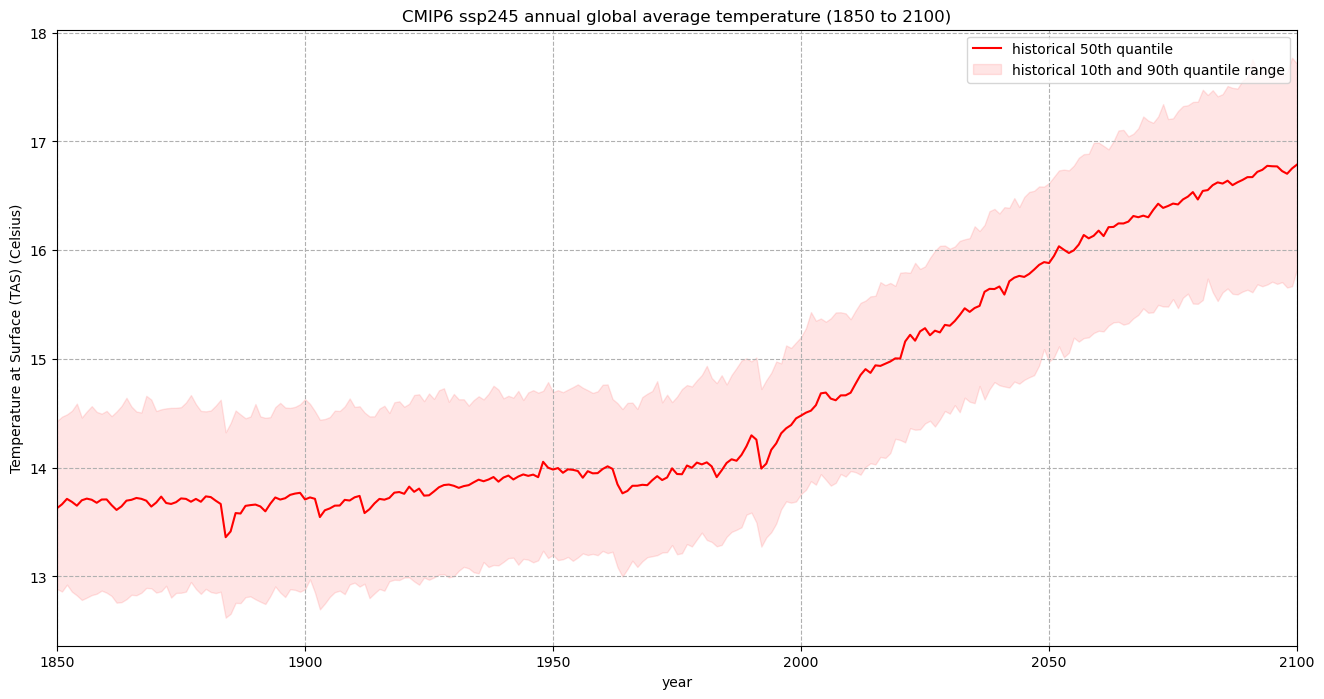
\includegraphics[width=7cm]{model_agg_global_avg_tas}
    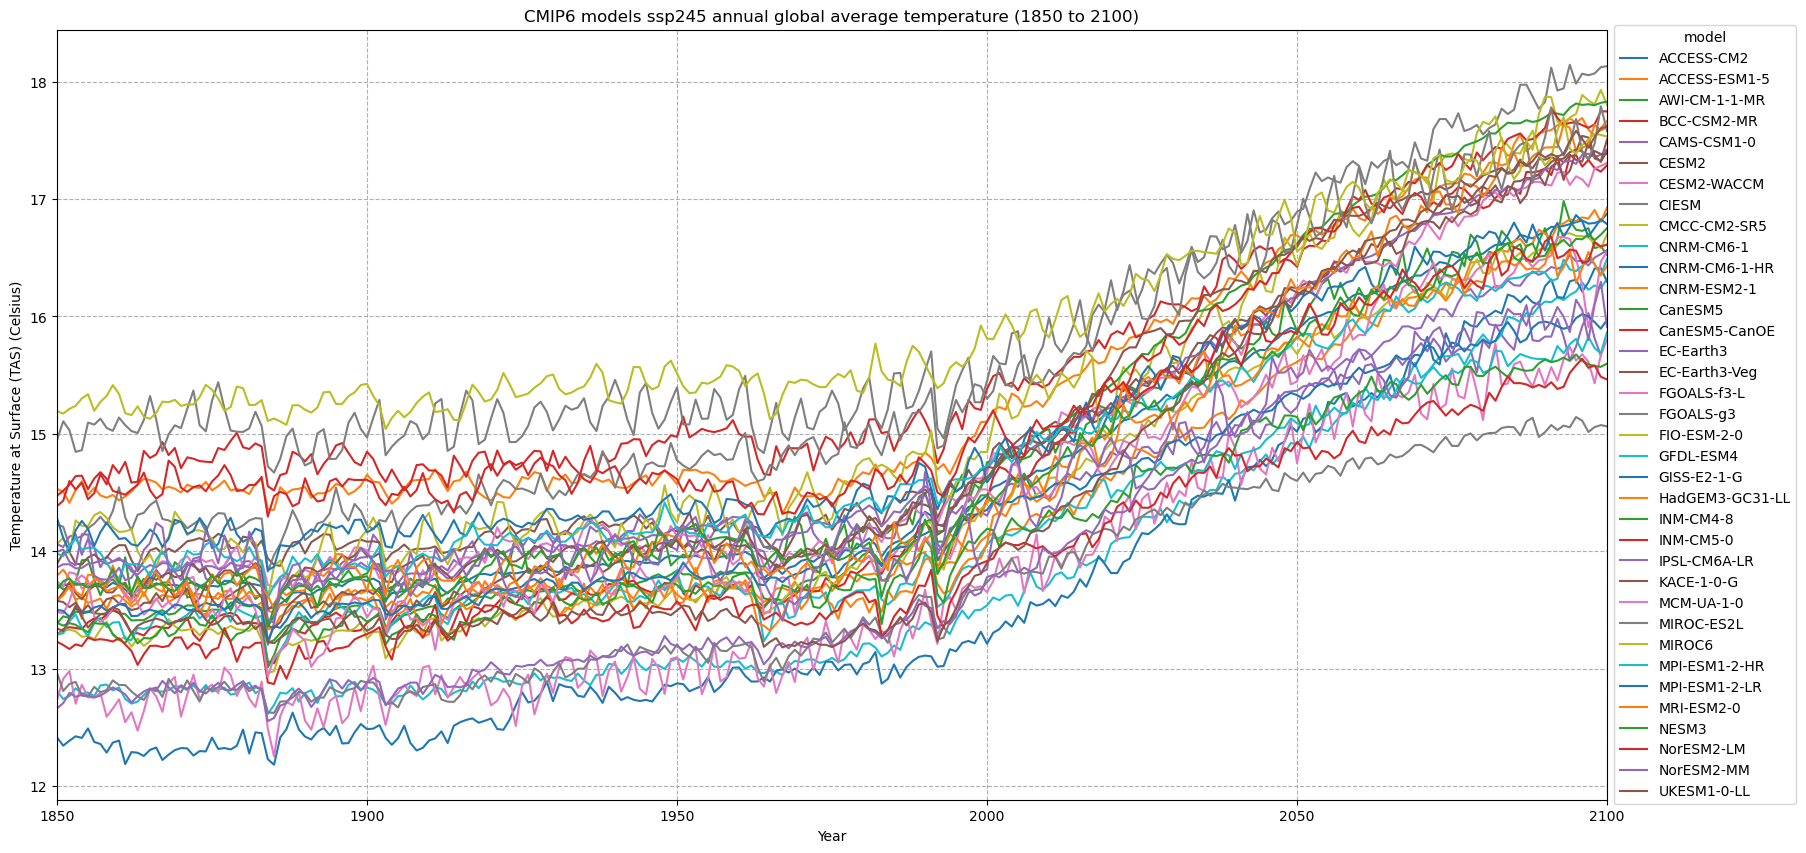
\includegraphics[width=7cm]{model_global_avg_tas}
    \centering
\end{figure}

Looking at a plot of all the models, there is a clear correlation between all the models and the correlation heatmap affirms this as the correlation between each
ranges from 0.96--1. 

\begin{figure}[t]
    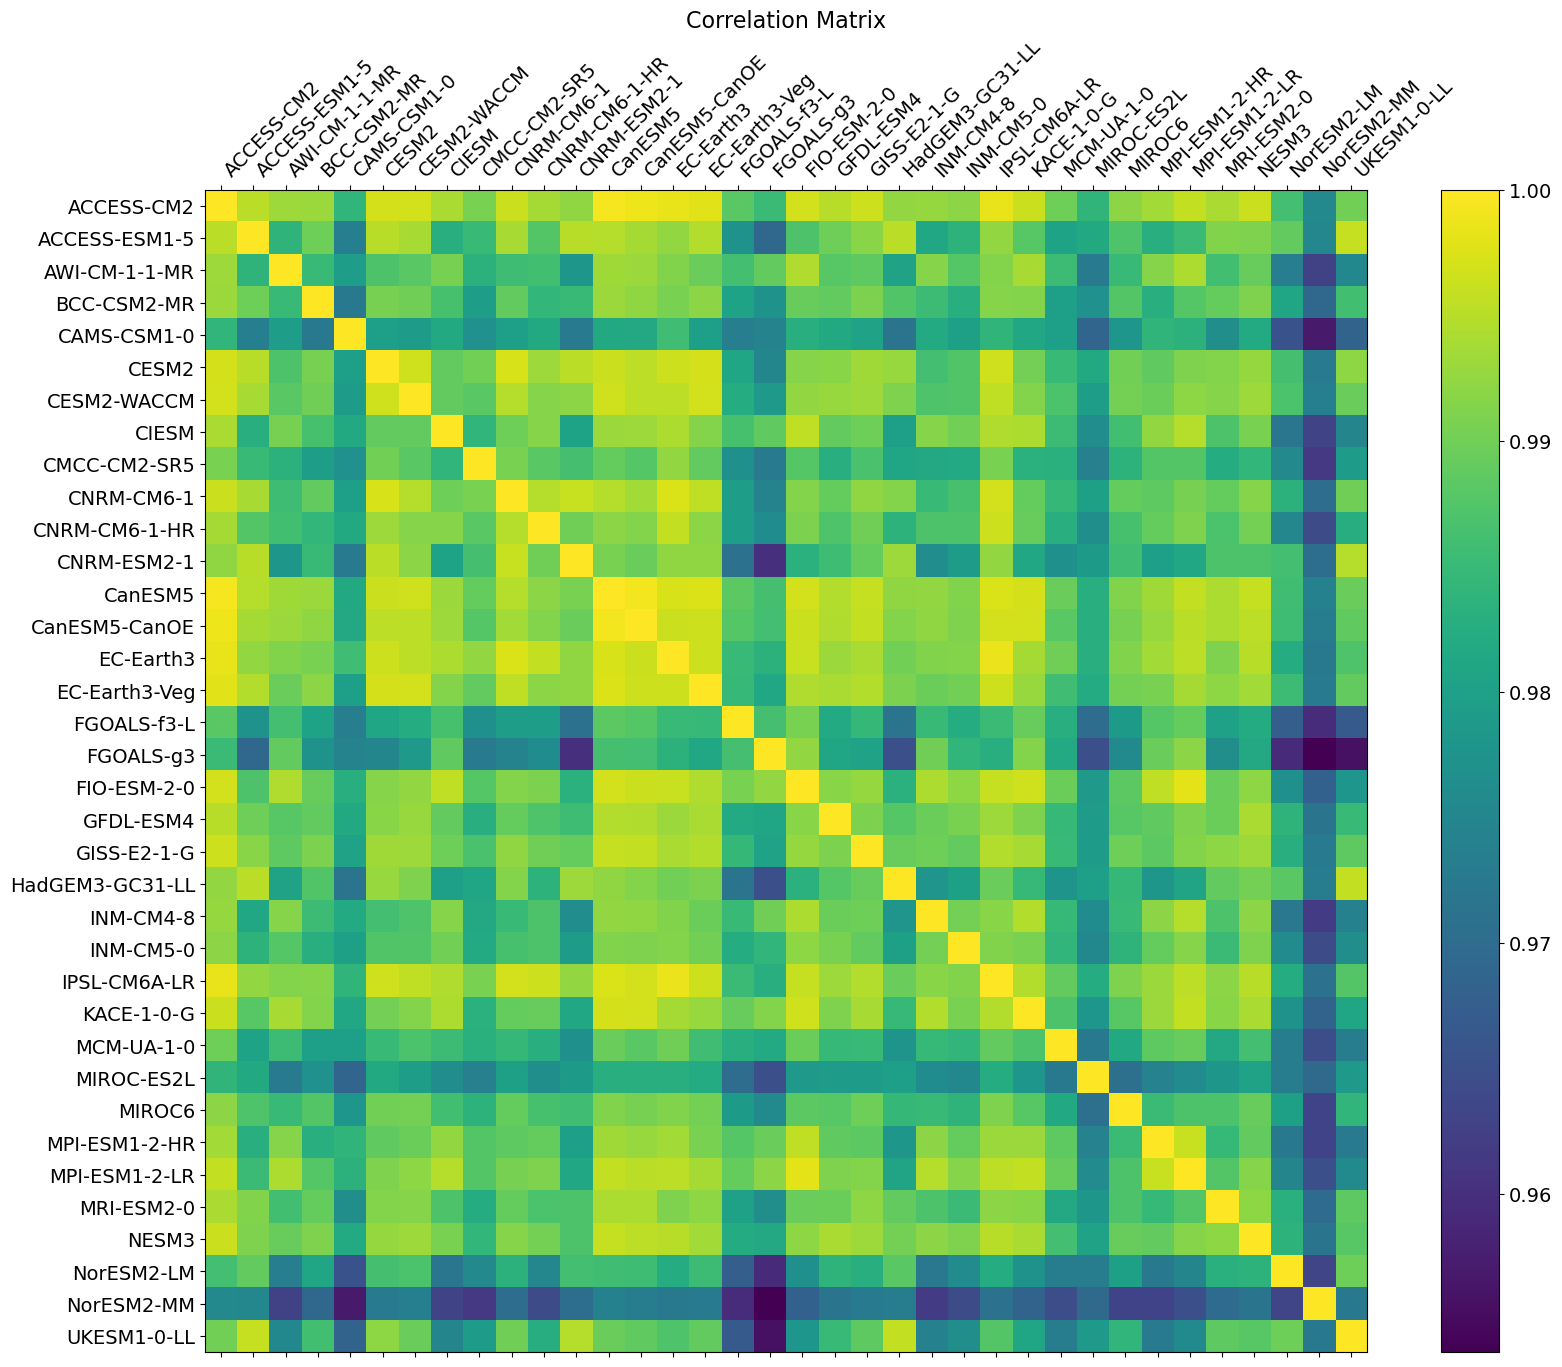
\includegraphics[width=10cm]{model_corr}
    \centering
\end{figure}

%%%%%%%%%%%%%%%%
\section{Dataset}\label{data}
The datasets used are from the CMIP6 scenario runs made available on the KNMI Climate Explorer website. The KNMI is part of the
World Meteoriological Organization (WMO)\cite{}. The scenario runs include monthly predictions for temperature, min temperature, max temperature
precipitation, radiation and pressure all over the globe in a 192$\times$144 grid between 1850--2100 for 40 different models. Due to the time and computational
limitations, this was filtered to just temperature during the 1960--1980 period in just Australia or latitudes -44{\textdegree} to -12{\textdegree} 
and longtitudes 288{\textdegree} to 336{\textdegree}. 

Talk a bit more about how these models in the dataset are all related by certain parts.
%%%%%%%%%%%%%%%%

{\section{Problem Formulation}}\label{problem-formulation}
\textit{Maybe add this to the background section and put more of the regression, diagrams of the process and shrinkage prior stuff here that it more specific to this thesis}

We define a graph as ${\mathcal{G}} = ({\mathcal{V}}, \textbf{A})$, where $\mathcal{V}$ represents a set of verticies which contains a list of nodes
$\{ v_1, \dots, v_n \}$ and $\textbf{A} \in \mathbb{R}^{n \times n}$ the adjacentcy matrix which contains information on the graph topology. If an edge exists
between two node $v_i$ and $v_j$, then $\textbf{A}_{ij} = 1$ else, $\textbf{A}_{ij} = 0$. We also define the degree matrix as $\mathbf{D} = \sum_{j}A_{ij}$
where each entry on the diagonal is equal to the row sum of the adjacency matrix $\textbf{A}$.  
Each node has a {p}-dimensional feature vector ${x_i} \in \mathbb{R}^{p}$
which describes some information about the node in the graph. By combining all ${n}$ feature vectors from all nodes, we have a feature matrix
$\textbf{X} \in \mathbb{R}^{n\times p}$. The graph also has a regression target ${Y} \in \mathbb{R}$ which refers to the historical temperature that each model from the
graph is attempting to predict. As mentioned earlier, other variables such as precipitation, pressure and radiation are available but for simplicity, just temperature
is currently being used. The two-layer GNN from \cite{kipf2017semisupervised} can be expressed as

\begin{equation}
f(\mathbf{A, X}) = \sigma_2( \mathbf{ \hat{A} }_2 \sigma_1 (\mathbf{ \hat{A} }_1 \mathbf{X} W^{(0)}) W^{(1)})
\end{equation}

\noindent where $\sigma_1(.)$ and $\sigma_2(.)$ are an activation function such as ReLU, and $\hat{A} = \tilde{D}^{-1/2} (A + I) \tilde{D}^{-1/2}$
is the symmetrically normalised adjacency matrix. The final regression problem can be formulated as

\begin{equation}
f : L \times X \rightarrow Y
\end{equation}

\noindent where $f$ denotes the learning function, $L$ the graph, $X$ denotes the time series input and $Y$ the regression target.

Need to describe the math behind graph sparsification. More about shrinkage see Xiongwens.

{\section{Computational features}}\label{computation}
computation of neural network models. See georges paper 
{\section{Implementation}}\label{implementation}

Need to finish code to finish this section.

\chapter{Results}\label{results}

{\section{Model verification}}\label{model-verification}
If the VGAE section is completed, we can compared the sparsified graph with the VGAE
produced graph to determine how good graph sparsification is when used for graph discovery
and thereby correlation in a graph structure.

{\section{Model results}}\label{model-results}
Is there some way we can test the models results depending on how sparse we make the graph etc.
Research required to find some quantitative measure for this.

Some figures of the NN structure would also be helpful for this.
Need to use nx or some other graph representation tool in python for this.

\chapter{Discussion}\label{dis}

\chapter{Conclusion}\label{ccl}

\chapter{Appendix}\label{app}


%%%%%%%%%%%%%%%%%%%%%%%%%%%%%%%%%%%%%%%%%%%%%%%%%%%%%%%%%%%%%%%%%%%%%%%%%%

\clearpage
\addcontentsline{toc}{chapter}{References}
\bibliography{bibliography}{}
\bibliographystyle{plain}

\end{document}





